\chapter{Introduction}

\section{Securing network}

\subsection{Terminologies}

An attack vector is a path or other means by which an attacker can gain access to a server, host, or network. Attack vectors can originate from outside (external threat) or inside (internal threat) the corporate network. Internal threats have the potential to cause greater damage than external threats because employees have direct access to infrastructure devices as well as the knowledge of the corporate network.\\

\textbf{White hat hackers} perform \emph{ethical} network penetration test to discover network vulnerabilities. \textbf{Grey hat hackers} do unethical things, but not for personal gain or to cause damage (e.g. disclose vulnerability publicly). \textbf{Black hat hackers} violate computer and network security for personal gain and malicious purposes. The following list displays modern hacking terms and a brief description of each.\\

\textbf{Security Artichoke} is the analogy used to describe what a hacker must do to launch an attack in a Borderless network. They  remove certain \emph{artichoke leafs}, and each \emph{leaf} of the network may reveal some sensitive data. And leaf after leaf, it all leads the hacker to more data.\\

\textbf{Cryptography} is the study and practice of hiding information. It ensures three components of information security: Confidentiality, Integrity, and Availability.\\

A \textbf{Security Policy} is a formal statement of the rules by which people that are given access to the technology and information assets of an organization, must abide.


\subsection{Network topology}

%\paragraph{Campus Area Networks:} The main focus of this course is on securing Campus Area Networks (CANs). CANs consists of interconnected LANs within a limited geographic area. Figure \ref{CANsec} displays a sample CAN with a defense in-depth approach using various security features and security devices to secure it.
%
%\begin{figure}[hbtp]
%\caption{CAN security}\label{CANsec}
%\centering
%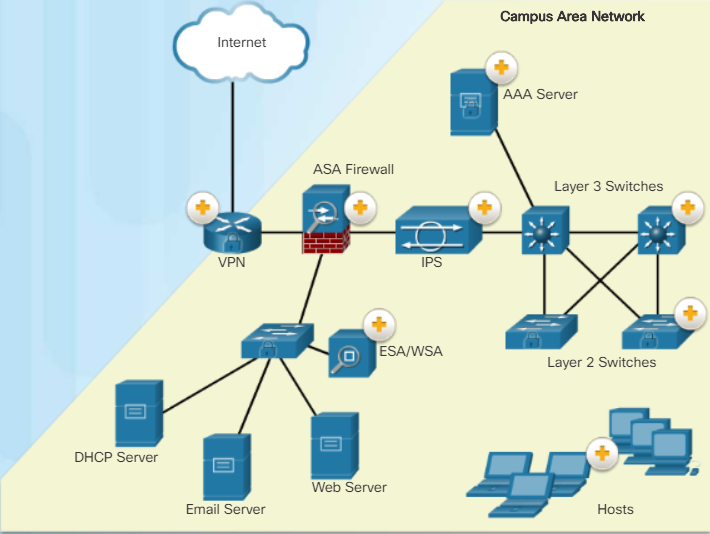
\includegraphics[scale=0.5]{pictures/CANsec.PNG}
%\end{figure}

\paragraph{SOHO network:} Attackers may want to use someone's Internet connection for free or illegal activity, or view financial transactions. Home networks and SOHOs are typically protected using a consumer \emph{grade router}, such as a \emph{Linksys home wireless router}. 

\paragraph{WAN network:} Main site and Regional site are protected by an ASA (stateful firewall and VPN). Branch site is secured using hardened ISR and VPN connection to the main site. The SOHO and Mobile users connect to the main site using Cisco Anyconnect VPN client. 

\paragraph{Data center network:} Data center networks are interconnected to corporate sites using VPN and ASA devices along with \emph{integrated data center switches}, such as a high-speed Nexus switches. Data center physical security can be divided into two areas: Outside perimeter security and Inside perimeter security. 
%\emph{Security traps} (Inside perimeter security) provide access to the data halls where data center data is stored. A person must first enter the security trap using their badge ID proximity card. After the person is inside the security trap, biometric verifications are used to open the second door. The user must repeat the process to exit the data hall.

\paragraph{Cloud and virtual network:} This kind of network uses virtual machines (VM) to provide services to their clients.  VMs are also prone to specific targeted attacks as shown in the following list. The \textbf{Cisco Secure Data Center} is a solution to secure Cloud and virtual network. The core components of this solution provide: Secure Segmentation, Threat Defense, and Visibility.

\begin{itemize}
\item \textbf{Hyperjacking:} An attacker could hijack a VM hypervisor and use it as a starting point to attack other devices.
\item \textbf{Instant on activation:} A VM that has not been used for a long period of time can introduce security vulnerabilities when activated.
\item \textbf{Antivirus storm:} Multiple VMs attempt to download antivirus file at the same time
\end{itemize}

\paragraph{Borderless Network:} To accommodate the BYOD trend, Cisco developed the Borderless Network. To support this network, Cisco devices support Mobile Device Management (MDM) features. MDM features secure, monitor, and manage mobile devices, including corporate-owned devices and employee-owned devices. 
%Some critical MDM functions include:
%
%\begin{itemize}
%\item Data encryption
%\item PIN enforcement
%\item Data wipe (data in lost devices can be remotely wiped out)
%\item Data Loss Prevention (DLP): prevent unauthorized users from accessing, prevent authorized users from doing malicious things to  critical data  
%\item Detect password bypasses such as Jalibreaking (Apple iOS) or Rooting (Android) and restrict devices' access to network and corporate assets
%\end{itemize}

\section{Network threats}

%\begin{itemize}
%\item Script kiddies -- inexperienced hackers running scripts, tools, programs, etc. to cause harm but not for profit
%\item Vulnerability broker -- white hat hackers discover exploits for reward
%\item Hacktivists -- protest against political or social ideas by leaking sensitive information
%\item Cyber criminals -- black hat hackers
%\item State-sponsored -- either white hat or black hat hacker, who steals government secrets, sabotage network, and intelligence; their targets are foreign government, terrorist group, and corporations
%\end{itemize}

%\subsection{Hacker tools}
%
%\begin{itemize}
%\item Password crackers -- repeatedly make guesses to crack the password; sometimes referred to as password recovery tool
%\item Wireless hacking tool
%\item Network scanning and hacking tools -- probe network devices for open TCP or UDP ports
%\item Packet crafting tool -- probe and test firewall's robustness
%\item Packet sniffer -- capture and analyze packets in Ethernet LAN or WLAN
%\item Rootkit detector -- used by white hat hackers to detect installed root kits
%\item Fuzzer -- discover computer's security vulnerability
%\item Forensic tools -- sniff out any trace of evidence existing
%\item Debuggers -- used by black hat hackers to reverse engineer binary files when writing exploits; used by white hat hackers to analyze malware
%\item Hacking OS -- designed OS preloaded with tools and technologies optimized for hacking, such as Kali Linux, SELinux, Knoppix, Backbox Linux
%\item Encryption tools
%\item Vulnerability scanners exploitation tool
%\item Vulnerability exploitation tool
%\end{itemize}
%
%Hackers can use the previously mentioned attack tools or a combination of tools to create various attacks. The figure displays common types of hacking attacks.
%
%\begin{itemize}
%\item Evesdropping
%\item Data modification
%\item IP address spoofing
%\item Password-based -- If hackers discover a valid account, they could obtain a list of other users, change configurations, etc.
%\item DoS
%\item Man-in-the-Middle: hackers position themselves between the source and destination to monitor, capture, and control communication
%\item Compromised key
%\end{itemize}

\subsection{Malware}

A \textbf{virus} is malicious code that is attached to executable files which are often legitimate programs. A virus is triggered by an event. When activated, the virus can infect all the files it has not yet infected, but does not automatically propagate itself to other systems. Viruses are \emph{spread} by USB memory drives, CDs, DVDs, network shares, and email. Email viruses are now the most common type of virus.\\

A \textbf{Trojan horse} is malware that carries out malicious operations under the guise of a desired function. A Trojan horse comes with malicious code hidden inside of it. This malicious code exploits the \emph{privileges} of the user that \emph{runs} it. Trojans are often found attached to online games. \\

\textbf{Worms} run by themselves, replicate and then spread very quickly (self-propagation) to slow down networks. They does not require user participation. After a host is infected, the worm is able to  over the network. Most worm attacks consist of three components:

\begin{itemize}
\item \textbf{Enabling vulnerability:} A worm installs itself using an exploit mechanism, such as an email attachment, an executable file, or a Trojan horse.
\item \textbf{Propagation mechanism:} After gaining access to a device, the worm replicates itself and locates new targets.
\item \textbf{Payload:} Any malicious code that results in some action is a payload. Most often this is used to create a backdoor to the infected host or create a DoS attack.
\end{itemize}

\note Worms never really stop on the Internet. After they are released, they continue to propagate until all possible sources of infection are properly patched.\\

Some other examples of modern malware:

\begin{itemize}
\item Ransomware -- deny access to the infected computer system, then demand a paid ransom for the restriction to be removed.
\item Spyware -- gather information about a user and send the information to another entity
\item Adware -- display annoying pop-up advertising pertinent to websites visited
\item Scareware -- include scam software which uses social engineering to shock or induce anxiety by creating the perception of a threat
\item Phishing -- attempt to convince people to divulge sensitive information, e.g. receiving an email from their bank asking users to divulge their account and PIN numbers.
\item Rootkits -- installed on a compromised system, then hide its intrusion and maintain privileged access to the hacker.
\end{itemize}

\subsection{Common network attacks}

The method used in this course classifies attacks in three major categories: Reconnaissance, Access, and DoS Attacks.\\

\textbf{Reconnaissance attacks} gather information about a network and scan for access. Some examples of reconnaissance attacks:  information query, ping sweep\footnote{a network scanning technique that indicates the live hosts in a range of IP addresses},  port scan,  Vulnerability Scanners,  Exploitation tools.\\

\textbf{Access attacks} exploit network vulnerabilities to gain access or control to sensitive information. There are five common types of access attacks: Password attack, Trust exploitation, Port redirection, Man-in-the-middle, Buffer overflow, IP spoofing, MAC spoofing, DHCP Spoofing.\\

\begin{itemize}
\item Password attack -- a dictionary is used for repeated login attempts
\item Trust exploitation -- uses granted privileges to access unauthorized material
\item Port redirection -- uses a compromised internal host to pass traffic through a firewall
\item Man-in-the-middle -- an unauthorized device positioned between two legitimate devices in order to redirect or capture traffic
\item Buffer overflow -- too much data sent to a buffer memory
\end{itemize}

%\textbf{Social engineering} is an \textbf{access attack} that attempts to manipulate individuals into performing actions or divulging confidential information. 
%Specific types of social engineering attacks include:
%
%\begin{itemize}
%\item Pretexting -- a hacker calls an individual and lies to them in an attempt to gain access to privileged data
%\item Phishing -- a malicious party sends a fraudulent email disguised as being from a legitimate, trusted source. The message intends to trick the recipient into installing malware on their device, or into sharing personal or financial information.
%\item Spam -- use spam email to trick a user to click an infected link or download an infected file.
%\item Tailgating -- This is when a hacker quickly follows an authorized person into a secure location. The hacker then has access to a secure area.
%\item Something for Something (Quid pro quo) -- a hacker requests personal information from a party in exchange for something like a free gift.
%\item Baiting -- a hacker leaves a malware-infected physical device, such as a USB flash drive in a public location such as a corporate washroom. The finder finds the device and loads it onto their computer, unintentionally installing the malware.
%\end{itemize}

\textbf{Denial-of-Service (DoS) attacks} prevent users from accessing a system. They are popular and simple to conduct. There are two major sources of DoS attacks:

\begin{itemize}
\item \emph{Maliciously Formatted Packets} is forwarded to a host and the receiver is unable to handle an unexpected condition, which leads to slow or crashed system.
\item \emph{Overwhelming Quantity of Traffic} causes the system to crash or become extremely slow.
\end{itemize}

\textbf{A Distributed DoS Attack (DDoS)} is similar in intent to a DoS attack, except that a DDoS attack increases in magnitude because it originates from multiple, coordinated sources. As an example, a DDoS attack could proceed as follows:

\begin{enumerate}
\item A hacker builds a network of infected machines. A network of infected hosts is called a \emph{botnet}. The compromised computers are called \emph{zombie computers}, and they are controlled by \emph{handler systems}.
\item The zombie computers continue to scan and infect more targets to create more zombies.
\item When ready, the hacker instructs the handler systems to make the botnet of zombies carry out the DDoS attack.
\end{enumerate}

\section{Mitigating Threats}

\subsection{Mitigating common network attacks}

\paragraph{Malware:} The primary means of mitigating virus and Trojan horse attacks is antivirus software. Antivirus software are host-based product that prevents hosts from getting infected and spreading malicious code. However, they do not prevent viruses from entering the network.

\paragraph{Worms:} They are more network-based than viruses. The response to a worm attack can be broken down into four phases:

\begin{enumerate}
\item \textbf{\textbf{Containment}:} limit the spread of worm infection
\item \textbf{Inoculation:} run parallel to or subsequent to the Containment phase; all uninfected systems are patched with the appropriate vendor patch.
\item \textbf{Quarantine:} identify the infected machines
\item \textbf{Treatment:} disinfect the infected systems
\end{enumerate}

\paragraph{Reconnaissance:} \emph{Encryption} is an effective solution for sniffer attacks. Using \emph{IPS} and \emph{firewall} can limit the impact of \emph{port scanning}. \emph{Ping sweeps} can be stopped if \emph{ICMP} echo and echo-reply are turned off on edge routers. 

\paragraph{Access attacks:} The network should be designed using the principle of minimum trust. This means that systems should not use one another unnecessarily. Other options are valid network security access protections (encrypted or hashed authentication protocols) but do not relate to the principle of minimum trust.

\paragraph{DoS attacks:} One of the first signs of a DoS attack is a large number of user complaints about unavailable resources. To minimize the number of attacks, a network utilization software and anti-spoofing technologies (port security, DHCP snooping, IP source guard, ARP inspection, and ACL) should be running at all times. 

\subsection{Cisco SecureX architecture}

The Cisco SecureX architecture is designed to provide effective security for any user, using any device, from any location, and at any time. This architecture includes the five major components: Scanning Engines, Delivery Mechanisms, Security Intelligence Operations (SIO), Policy Management Consoles, and Next-Generation Endpoints. The most important component of SecureX is SIO, which detects and blocks malicious traffic.\\

The SecureX is a huge and complex computing model. Therefore, a \textbf{context-aware scanning element} is used to scale SecureX. It is a device that examines packets as well as external information to understand the full context of the situation. To be accurate, this context-aware device defines security policies based on five parameters: person ID, application, device type, location, and access time.\\

\textbf{Security Intelligence Operations (SIO)} is a Cloud-based service that connects global threat information, reputation-based services, and sophisticated analysis, to SecureX network security devices.

\subsection{Cisco Network Foundation Protection Framework}

The Cisco Network Foundation Protection (NFP) framework provides comprehensive guidelines for protecting the network infrastructure.  NFP logically divides routers and switches into three functional areas: Control plane, Management plane, and Data plane.\\

\begin{itemize}

\item\textbf{Control plane} is responsible for routing functions. Its security is implemented by Routing protocol authentication, CoPP, and AutoSecure. CoPP (Control Plane Policing) prevents unnecessary traffic from overwhelming the route processor. \textbf{AutoSecure} can lock down the management plane functions and the forwarding plane services and functions of a router.\\

\item\textbf{Management plane} is responsible for network security and management. Its security is implemented by password policy, RBAC\footnote{Role-based access control  restricts user access based on the role of the user. In Cisco IOS, the role-based CLI access feature implements RBAC for router management access.}, authorization, access reporting.

\item\textbf{Data plane} (Forwarding plane) is responsible for forwarding data. Its security can be implemented using \emph{ACLs}, \emph{antispoofing mechanisms}, and \emph{Layer 2 security} features. 

\end{itemize}
%\begin{itemize}
%\item ACLs are used to secure the data plane in a variety of ways: Blocking unwanted traffic or users, Reducing the chance of DoS attacks, Mitigating spoofing attacks, Providing bandwidth control, Classifying traffic to protect the Management and Control planes.
%\item Layer 2 security tools are integrated into the Cisco Catalyst switches: Port security, DHCP snooping, Dynamic ARP Inspection (DAI), and IP Source Guard.
%\end{itemize}